% cs434-sp17 final paper, hoeftc and gillenp
% based on nips_2017.tex

\documentclass{article}

% if you need to pass options to natbib, use, e.g.:
% \PassOptionsToPackage{numbers, compress}{natbib}
% before loading nips_2017
%
% to avoid loading the natbib package, add option nonatbib:
% \usepackage[nonatbib]{nips_2017}

% print author's names
\usepackage[final]{nips_2017}

\usepackage[utf8]{inputenc} % allow utf-8 input
\usepackage[T1]{fontenc}    % use 8-bit T1 fonts
\usepackage{hyperref}       % hyperlinks
\usepackage{url}            % simple URL typesetting
\usepackage{booktabs}       % professional-quality tables
\usepackage{amsfonts}       % blackboard math symbols
\usepackage{nicefrac}       % compact symbols for 1/2, etc.
\usepackage{microtype}      % microtypography
\usepackage{mathtools}
\usepackage{caption}

\title{Finding Quora questions pairs with neural networks}

% The \author macro works with any number of authors. There are two
% commands used to separate the names and addresses of multiple
% authors: \And and \AND.
%
% Using \And between authors leaves it to LaTeX to determine where to
% break the lines. Using \AND forces a line break at that point. So,
% if LaTeX puts 3 of 4 authors names on the first line, and the last
% on the second line, try using \AND instead of \And before the third
% author name.

\author{
    Cody Ray Hoeft \\
    School of EECS \\
    Oregon State University \\
    Corvallis, OR 97331 \\
    \texttt{hoeftc@oregonstate.edu} \\
    \And
    Padraig Gillen \\
    School of EECS \\
    Oregon State University \\
    Corvallis, OR 97331 \\
    \texttt{gillenp@oregonstate.edu} \\
}

\begin{document}
% \nipsfinalcopy is no longer used

\maketitle

\begin{abstract}
    Anybody can ask and answer questions on Quora, the question answer site. With 100 million monthly users, questions with the same intent are frequently asked. Questions with the same intent can lead to more overhead for Quora, readers, and writers. Quora challenged the Kaggle Community to find a better way to identify question pairs. We started with a starter Kernel from the Kaggle Community and experimented with changing the word embedding and trying different neural networks.
\end{abstract}

\section{Introduction}
% An introduction section that briefly describes the problem you aimed to solve and a summary of the main results

	The goal of the Quora question pairs challenge was to determine if two questions were duplicate, that is they shared the same intent. Quora provided a training set of over $.4$ million questions, each labeled as a duplicate or not a duplicate. Quora also provided a testing set of over $2.3$ million unlabeled questions of for judging the competition. The goodness of an algorithm was evaluated by log loss. Kaggle returns the log loss as a score after uploading the predicted labels for the test data.
    
    We started with a Long Short-Term Memory (LSTM) neural network using word2vec embeddings based on Python code from Kaggle user lystdo (``LSTM with word2vec embeddings'') but with some of the code for cleaning text removed. This achieved a score of $0.30907$, but we wanted to know if we could do better with other word embeddings, a Gated Recurrent Unit (GRU) network, or Convolutional Neural Network (CNN).
    
    We were unable to improve performance much beyond the initial code, but we had the opportunity to experiment with different approaches and found that given the same features most yielded comparable results. We found that Convolutional Neural Networks performed surprisingly well even when only using the letters of the question (without any pretrained model).

\section{Approach}
% One / multiple sections describing the approach(es) you explored for solving the problem.
% Examples: feature design, preprocessing, and the prediction models etc.

\subsection{Preprocessing}

Various methods of preprocessing the questions were investigated. To be used with word embeddings, words must be identified within the sentence. The simplest preprocessing  is to split the sentence into words using white space. The weakness is that some punctuation can cause words to be different even though they are the same; for example, ``love?'' and ``love'' should be interpreted as the same word. Striping punctuation. Replacing punctuation with spaces (except for apostrophe) makes words touching punctuation the same. The capitalization of words can also cause words to be different, so words are made lowercase. Stop words are words so common that they carry no extra meaning and can be removed from the sentence. Additionally, some words have the same roots but are syntactically different, i.e., `remove' and `removing'. Stemming can be used to convert both words to the same word. Additionally, many words in the training and testing set are misspelled. Automatic spell checking could correct the misspelled words.

\subsection{Different Word Embeddings}

Text data by itself doesn't contain much meaningful data. Word embeddings map words to vectors that have more meaning than the text itself. Building embeddings requires extremely large corpuses because they are finding a mapping from sparse data to dense data. Because the provided training and testing data are too small to train embeddings, we did not attempt to train one from scratch. Instead we tried using pretrained models including a model trained on a Google News corpus and Glove embeddings trained on a variety of sources.

Attempts were also made to improve the embeddings themselves. The embeddings contain both capitalized words and lowercase words. For example, ``Trump'' and ``trump'' both exist in the Google News embeddings, but `Trump' will have occurred more in the corpus and therefore the vector should have more meaning. Since preprocessed sentences can never contain capital words, we can remap ``Trump'' to ``trump'' and discard the original ``trump''. Likewise, words that cannot possibly exist in the preprocessed sentences can be discarded to improve load time of the embeddings.

\subsection{Different Neural Networks}

\begin{center}
  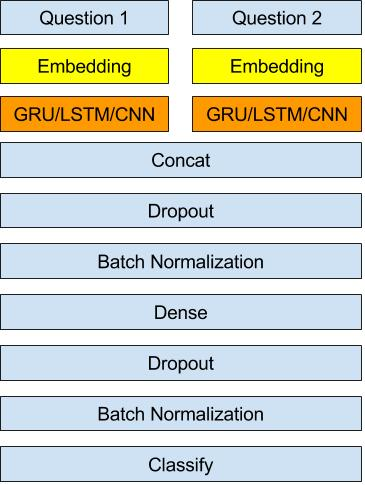
\includegraphics[width=0.4\textwidth]{NeuralNetStructure}
  \captionof{figure}{Outline of the structure used for GRU, LSTM, and CNN neural networks}
  \label{nns}
\end{center}

The structure used in Figure~\ref{nns} was used to support three distinct types of neural networks which replace the orange block in the neural network.

A Long Short-Term Memory (LSTM) network is a typical way to perform sentiment analysis on text. An LSTM is a reasonable choice for this problem because recognizing similar intent in a question is comparable to sentiment analysis.

A Gated Recurrent Unit (GRU) network is like an LSTM with similar performance but has fewer internal parameters to train.

A Convolutional Neural Network (CNN) is a network made of filters that is commonly used in image processing. A CNN is a reasonable choice for this problem because it has the potential to extract similarities in the sentences in various parts of the sentences.

\begin{center}
  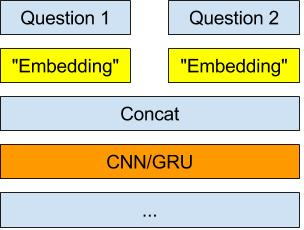
\includegraphics[width=0.35\textwidth]{LetterNeuralNetStructure}
  \captionof{figure}{Outline of the structure used for letter-wise neural networks}
  \label{lnns}
\end{center}

In addition to the original structure, which used word embeddings. CNN and GRU neural nets were also attempted over letters instead of words. As shown in Figure~\ref{lnns}, the location in the neural network where the two paths were concatenated was also moved before the CNN layer. To enable the encoding of the letters a 2 dimension word2vec instance was trained from scratch using each letter as a word. After the embedding each letter, the 2d vectors for each letter are joined into a 4d vector pairwise for the first 150 letters.

\section{Results}
% section devoted to presenting / discussing the results  obtained from exploration
% possible discussion topics include:
%   what worked and what didn't?
%   How do different methods compare with each other?

\subsection{Preprocessing}

Stripping punctuation and making the sentence lowercase improved the validation loss. However, removing stop words and stemming were found to make the validation loss worse. Automatic spell check with a method explained on Kaggle, was attempted; but was found to be too resource intensive.

\subsection{Word Embeddings}

There was only a small difference between the validation loss of models trained on the Google News corpus and the Glove embeddings. In general, the Google News vectors performed better however the test loss difference was smaller than the test loss difference between the same model being run with different validation splits.

Efforts to improve the embeddings themselves yielded very small improvements in test loss. For Google News, the improvement was $0.00548$ and for Glove the improvement was $0.00095$. However, the size of the embeddings were reduced by $0.47$ GB and $1.22$ GB respectively. This helps them load faster.

\subsection{Different Neural Networks}

We started with an LSTM network which achieved a score of $0.30802$ using Glove embeddings. The GRU network achieved a slightly better score of $0.30411$. The CNN network was less successful, with a score of $0.33798$.

The letter-wise GRU network failed to get less than a loss of $0.4$ after several epochs of training. However, the letter-wise CNN worked surprisingly well and yielded a score of $0.36233$.

\subsection{Lessons Learned}
%   what kind of lessons you learned from your exploration?
%   What are possible ways for future work to improve?

As this was a project for an introductory class, most of our learning came in understanding the existing models and frameworks used in the field of machine learning. We learned a lot about the Python libraries available like \texttt{keras}, but found they obscured a lot of the details necessary to quickly see past the ``magic''.

We also learned that changing models often doesn't bring much in the way of accuracy gains, though it can speed up model loading and processing times. After reading the discussions by the winners of the Kaggle competitions, we noticed how important feature engineering is, and how finding the right combination will beat out na\"{\i}ve learning even with powerful tools.

For this to be most effective requires in-depth research into the datasets, trail and error with parameters, and a powerful computing platform to give rapid feedback. If we had a chance to work on this more, we would focus on longer training sessions for the letter-wise CNN, as well as looking for other patterns we didn't have time to explore, like TF-IDF.


\section{Conclusion}
% A conclusion section that summarize your project and your effort.

In this project, we gained a practical exposure to LSTM, GRU, and CNN networks. We also got a chance to start testing our implementation quickly with embeddings, instead of making a best guess start like previous assignments. This allowed us to get a sense for training and testing accuracy within a few epochs, even on resource constrained systems.

This project was challenging to implement, and required a lot of time handling programming logic and server errors before we could dive into model analysis. However, it was rewarding to see how accessible the field is, and how we could tackle a hard problem with a comparatively small amount of code. We have enjoyed working with language processing as relative novices, and achieving fairly good accuracy in classification. Though we have more questions now than at the start, this project has provided a great foundation into practical machine learning, and should serve us well as we work on classification problems going forward. 




\clearpage
\appendix
\section{Work Done}
% appendix describes individual contribution levels to the project
%    estimated in percentages and described in words
\subsection{Kaggle user ``lystdo''}
Without ``lystdo'' we wouldn't have been able to accomplish as much as we did, we learned a lot from his starter code.
% Is it silly to leave this in here?
% haha, I think it's good to have

\subsection{Padraig Gillen}
After a slow start to the project due to a high course load, Padraig focused on getting up to speed with the existing project code base, and started the documentation. He worked with IT staff on reproducing and solving the CPU deadlock issue we encountered, but these proved mostly unfruitful as a minimal working example was hard to produce, and the shared server could not be restarted often.

Later work involved edits to the presentation and report for grammar and clarity, and writing the final sections of the report. Total work done was around $35\%$.

\subsection{Cody Ray Hoeft}
Cody had a \textit{very} light class load and an idle GPU. He was perhaps a little too eager to get started on the project and did some of the early experimentation with the LSTM after figuring out how to run keras on his Desktop computer. He also came up with the idea to clean the word2vec files to speed up their loading. Total work was around $65\%$

\end{document}

% \subsection{Citations within the text}
%
% The \verb+natbib+ package will be loaded for you by default.
% Citations may be author/year or numeric, as long as you maintain
% internal consistency.  As to the format of the references themselves,
% any style is acceptable as long as it is used consistently.
%
% The documentation for \verb+natbib+ may be found at
% \begin{center}
%     \url{http://mirrors.ctan.org/macros/latex/contrib/natbib/natnotes.pdf}
% \end{center}
% Of note is the command \verb+\citet+, which produces citations
% appropriate for use in inline text.  For example,
% \begin{verbatim}
%     \citet{hasselmo} investigated\dots
% \end{verbatim}
% produces
% \begin{quote}
%     Hasselmo, et al.\ (1995) investigated\dots
% \end{quote}
%
% If you wish to load the \verb+natbib+ package with options, you may
% add the following before loading the \verb+nips_2017+ package:
% \begin{verbatim}
%     \PassOptionsToPackage{options}{natbib}
% \end{verbatim}
%
% If \verb+natbib+ clashes with another package you load, you can add
% the optional argument \verb+nonatbib+ when loading the style file:
% \begin{verbatim}
%     \usepackage[nonatbib]{nips_2017}
% \end{verbatim}
%
% As submission is double blind, refer to your own published work in the
% third person. That is, use ``In the previous work of Jones et
% al.\ [4],'' not ``In our previous work [4].'' If you cite your other
% papers that are not widely available (e.g., a journal paper under
% review), use anonymous author names in the citation, e.g., an author
% of the form ``A.\ Anonymous.''
%
%
% \subsection{Tables}
%
% All tables must be centered, neat, clean and legible.  The table
% number and title always appear before the table.  See
% Table~\ref{sample-table}.
%
% Place one line space before the table title, one line space after the
% table title, and one line space after the table. The table title must
% be lower case (except for first word and proper nouns); tables are
% numbered consecutively.
%
% Note that publication-quality tables \emph{do not contain vertical
%   rules.} We strongly suggest the use of the \verb+booktabs+ package,
% which allows for typesetting high-quality, professional tables:
% \begin{center}
%   \url{https://www.ctan.org/pkg/booktabs}
% \end{center}
% This package was used to typeset Table~\ref{sample-table}.
%
% \begin{table}[t]
%   \caption{Sample table title}
%   \label{sample-table}
%   \centering
%   \begin{tabular}{lll}
%     \toprule
%     \multicolumn{2}{c}{Part}                   \\
%     \cmidrule{1-2}
%     Name     & Description     & Size ($\mu$m) \\
%     \midrule
%     Dendrite & Input terminal  & $\sim$100     \\
%     Axon     & Output terminal & $\sim$10      \\
%     Soma     & Cell body       & up to $10^6$  \\
%     \bottomrule
%   \end{tabular}
% \end{table}
